\documentclass[a4paper, 12pt]{article}%тип документа

%отступы
\usepackage[left=2cm,right=2cm,top=2cm,bottom=3cm,bindingoffset=0cm]{geometry}
\setlength{\parindent}{5ex}

%Русский язык
\usepackage[T2A]{fontenc} %кодировка
\usepackage[utf8]{inputenc} %кодировка исходного кода
\usepackage[english,russian]{babel} %локализация и переносы

%Вставка картинок
\usepackage{graphicx}
\graphicspath{{pictures/}}
\DeclareGraphicsExtensions{.pdf,.png,.jpg}

%Графики
\usepackage{pgfplots}
\pgfplotsset{compat=1.9}

%Математика
\usepackage{amsmath, amsfonts, amssymb, amsthm, mathtools}

%Таблицы
\usepackage{longtable} 
\usepackage{float}

%Римские цифры
\newcommand{\RomanNumeralCaps}[1]{\uppercase\expandafter{\romannumeral#1}}

\usepackage{multirow}


\begin{document}
	\begin{titlepage}
		\begin{center}
			\textsc{Федеральное государственное автономное образовательное учреждение высшего образования«Московский физико-технический институт (национальный исследовательский университет)»\\[5mm]
			}
			
			\vfill
			
			\textbf{Отчёт по лабораторной работы 3.4.1\\[3mm]
				Диа- и парамагнетики
				\\[50mm]
			}
			
		\end{center}
		
		\hfill
		\begin{minipage}{.5\textwidth}
			Выполнил студент:\\[2mm]
			Сериков Василий Романович\\[2mm]
			группа: Б03-102\\[5mm]
			
		\end{minipage}
		\vfill
		\begin{center}
			Москва, 2022 г.
		\end{center}
		
	\end{titlepage}
	
	\newpage
	\textbf{Аннотация}\\
	
	
	\textbf{Цель работы: }\\
	
	Измерение магнитной восприимчивости диа- и парамагнитного образцов.\\
	
	\textbf{В работе используются: }\\
	
	Электромагнит, электронные весы, милливеберметр, регулируемый источник постоянного тока, образцы.\\
	
	\textbf{Теоретические сведения: } \\
	
	Магнитная восприимчивость тел может быть определена по измерению сил, действующих на тела в магнитном поле. В данной работе измерения проводятся классическим методом Гюи. Суть этого метода состоит в использовании тонкого и длинного стержня, один из концов которого помещают в зазор электромагнита (обычно в область однородного поля), а другой конец — вне зазора, где величиной магнитного поля можно пренебречь. Закон изменения поля — от максимального до нулевого — в этом случае несуществен.
	
	\begin{figure}[h]
		\center{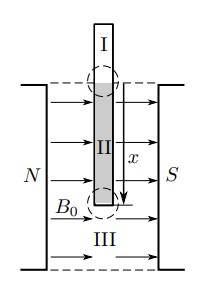
\includegraphics [scale=1]{photo1.png}}
		\caption{Схема для вывода формулы.}
	\end{figure}
	
	При смещении образца на расстояние $ dx $ магнитная сила, действующая на него, равна
	
	\begin{equation}\label{1}
		F = \left(\frac{\partial W}{\partial l}\right)_I,
	\end{equation}
	где $ dW $ -- изменение магнитной энергии системы при постоянном токе
	в обмотке электромагнита и, следовательно, при постоянной величине
	магнитного поля в зазоре.
	
	Магнитная энергия рассчитывается по формуле
	
	\begin{equation}\label{2}
		W=\frac{1}{2}\int HBd\,V = \frac{1}{2\mu_0}\int\frac{B^2}{\mu}d\,V,
	\end{equation}
	где интеграл распространён на всё пространство. При смещении образца магнитная энергия меняется только в области зазора (в объёме площади $ s $ и высоты $ dx $), а около верхнего конца стержня остаётся неизменной, поскольку магнитного поля там практически нет. В области $\RomanNumeralCaps{1}$ вне электромагнита поле мало
	$B_1 = 0$ и его вкладом в энергию можно пренебречь.
	В части стержня $\RomanNumeralCaps{2}$, погружённой в электромагнит,
	поле приближённо равно $B_2 = \mu B_0$. В области $\RomanNumeralCaps{3}$
	вдали от стержня поле мало отличается от $B_3 = B_0$, получим
	
	\begin{equation}\label{3}
	dW=\frac{1}{2\mu_0}\frac{B^2_2}{\mu}Sdx - \frac{1}{2\mu_0}B^2_3 Sdx = -\frac{(\mu - 1)}{2\mu_0}B^2_0Sdx.
	\end{equation}
	
	Следовательно, на образец действует сила
	
	\begin{equation}\label{4}
		F = -\frac{\chi}{2\mu_0}B^2_0S.
	\end{equation}
	
	Знак силы, действующей на образец, зависит от знака $ \chi $: образцы из парамагнитных материалов $( \chi  > 0)$ втягиваются в зазор электромагнита, а диамагнитные образцы $ (\chi < 0) $ выталкиваются из него. Измерив силу, действующую на образец в магнитном поле $ B_0 $, можно рассчитать магнитную восприимчивость образца.\\
	
	\textbf{Экспериментальная установка и методика измерений: }\\
	
		\begin{figure}[h]
		\center{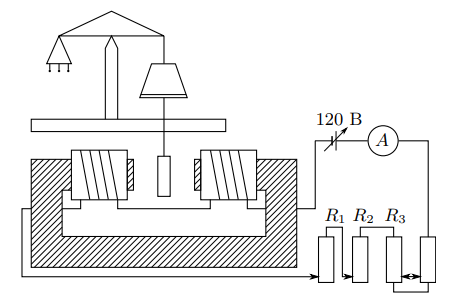
\includegraphics [scale=1]{photo2.png}}
		\caption{Схема экспериментальной установки.}
	\end{figure}
	
	Схема установки изображена на рис. 2. Магнитное поле с максимальной индукцией $\approx $1 Тл создаётся в зазоре электромагнита, питаемого
	постоянным током. Диаметр полюсов существенно превосходит ширину зазора, поэтому поле в средней части зазора достаточно однородно.
	Величина тока, проходящего через обмотки электромагнита, задаётся
	регулируемым источником постоянного напряжения.
	Градуировка электромагнита (связь между индукцией магнитного
	поля B в зазоре электромагнита и силой тока I в его обмотках) производится при помощи милливеберметра.\\
	
	При измерениях образцы поочерёдно подвешиваются к весам так, что один конец образца оказывается в зазоре электромагнита, а другой — вне зазора, где индукцией магнитного поля можно
	пренебречь. При помощи весов определяется перегрузка $\Delta P = F$ — сила, действующая на образец со стороны магнитного
	поля.\\
	
	\textbf{Результаты измерений и обработка данных: }\\
	\begin{enumerate}
	
	\item Начальные данные и погрешности.\\
	$SN$ = 72см$^2$ - произведение площади сечения пробной катушки на число
	витков в ней.\\
	$\sigma_{mWb}$ = 0,1 мВб - систематическая погрешность измерения потока $\Phi$.\\
	$\sigma_{A}$ = 0,05 А - систематическая погрешность измерения силы тока.\\
	$d_{Cu} = 10,10 \pm 0,05$ мм - диаметр медного стержня.\\
	$d_{Al} = 9,90 \pm 0,05$ мм - диаметр алюминиево стержня.\\
	
	\item Проведем градуировку электромагнита. Для этого с помощью милливеберметра снимем зависимость магнитного потока $\Phi$, пронизывающего пробную катушку, находящуюся в зазоре, от тока $I (\Phi = BSN)$ $\varepsilon_B = \varepsilon_\Phi => \sigma_B \approx 13$ мТл. Полученные данные занесем в таблицу 1.
	
	\begin{longtable} {|c|c|c|c|c|c|c|c|c|}
		\hline
		№ & 1 & 2 & 3 & 4 & 5 & 6 & 7 & 8 \\ \hline 
		$I, $ А & 0 & 0,4 & 0,8 & 1,2 & 1,6 & 2,0 & 2,4 & 2,8 \\ \hline
		$\Phi, $ мВб & 0,3 & 0,65 & 1,25 & 1,6 & 2,0 & 2,65 & 3,1 & 3,4 \\ \hline
		$B, $ мТл & 42 & 90 & 173 & 222 & 277 & 368 & 430 & 472 \\ \hline
	\caption{Результаты измерений $\Phi$}
	\end{longtable}
	
	\item По полученным данным построим градуировочную прямую $B(I)$
	
	\begin{figure}[h]
		\center{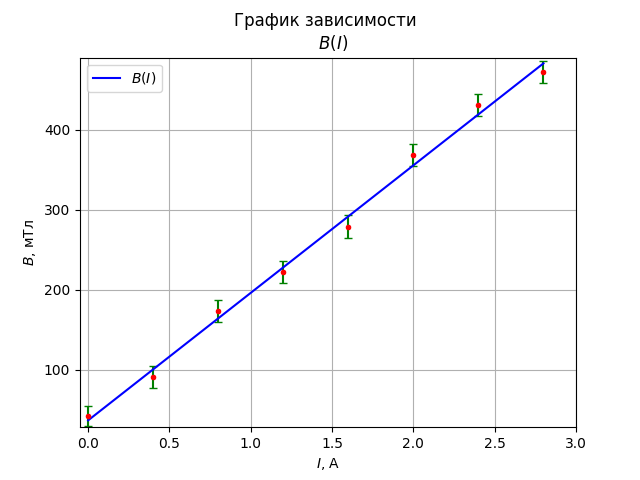
\includegraphics [scale=1]{3-4-1_first.png}}
		\caption{График зависимости $B(I)$}
	\end{figure}
	
	\item Измерим силы, действующие на образцы меди и алюминия в магнитном поле. Запишем полученные значения в таблицы 2 и 3. ($\varepsilon_{\Delta P} = \varepsilon_m \approx 1 \cdot 10^{-5}  << \varepsilon_{B^2} = 2\varepsilon_{B}$)
	
	\begin{longtable} {|c|c|c|c|c|c|c|c|c|}
		\hline
		№ & 1 & 2 & 3 & 4 & 5 & 6 & 7 & 8 \\ \hline 
		$I, $ А  $\nearrow$ & 0 & 0,4 & 0,8 & 1,2 & 1,6 & 2,0 & 2,4 & 2,8 \\ \hline
		$\Delta P, \cdot 10^{-5}$ Н  & 0 & 2,0 & 4,9 & 9.8 & 16,6 & 24,5 & 33,3 & 43,1 \\ \hline
		$B^2, \cdot 10^{-3}$ Тл$^2$ & 1,7 & 8,2 & 30,1 & 49,4 & 77,1 & 135,5 & 185,4 & 222,9 \\ \hline
		\hline
		$I, $ А  $\searrow$ & 0 & 0,4 & 0,8 & 1,2 & 1,6 & 2,0 & 2,4 & 2,8 \\ \hline
		$\Delta P, \cdot 10^{-5}$ Н  & 0 & 2,0 & 3,9 & 9,8 & 17,6 & 23,5 & 32,3 & 40,1 \\ \hline
		$B^2, \cdot 10^{-3}$ Тл$^2$ & 1,7 & 8,2 & 30,1 & 49,4 & 77,1 & 135,5 & 185,4 & 222,9 \\ \hline
		\caption{Результаты измерений для алюминиево стержня при увеличении и уменьшении I.}
	\end{longtable}
	
	\begin{longtable} {|c|c|c|c|c|c|c|c|c|}
		\hline
		№ & 1 & 2 & 3 & 4 & 5 & 6 & 7 & 8 \\ \hline 
		$I, $ А  $\nearrow$ & 0 & 0,4 & 0,8 & 1,2 & 1,6 & 2,0 & 2,4 & 2,8 \\ \hline
		$\Delta P, \cdot 10^{-5}$ Н  & 0 & -1,0 & -2,0 & -3,9 & -6,8 & -10,7 & -14,7 & -18,6 \\ \hline
		$B^2, \cdot 10^{-3}$ Тл$^2$ & 1,7 & 8,2 & 30,1 & 49,4 & 77,1 & 135,5 & 185,4 & 222,9 \\ \hline
		\hline
		$I, $ А  $\searrow$ & 0 & 0,4 & 0,8 & 1,2 & 1,6 & 2,0 & 2,4 & 2,8 \\ \hline
		$\Delta P, \cdot 10^{-5}$ Н  & 0 & -1,0 & -2,0 & -4,9 & -8,8 & -12,7 & -17,6 & -20,5 \\ \hline
		$B^2, \cdot 10^{-3}$ Тл$^2$ & 1,7 & 8,2 & 30,1 & 49,4 & 77,1 & 135,5 & 185,4 & 222,9 \\ \hline
		\caption{Результаты измерений для медного стержня при увеличении и уменьшении I.}
	\end{longtable}

	
	\item Построим графики зависимости $|\Delta P| (B^2)$ для меди и алюминия. По графикам определим коэффициент наклона прямых и рассчитаем магнитную восприимчивость $\chi$ по формуле (4). $\varepsilon_{	\frac{\Delta P}{B^2}} = \varepsilon_{B^2} = 2\varepsilon_{B} = 0,3 >> \varepsilon_{\frac{\Delta P}{B^2}}^{\text{мнк}}$
	
	\begin{equation}
		\frac{\Delta P}{B^2} = \frac{\chi}{2\mu_0}S.
	\end{equation}

	\begin{equation}
		\chi = \frac{\Delta P}{B^2}\frac{2\mu_0}{\rho S}.
	\end{equation}

	\begin{equation}
		\sigma_{\chi} = \chi\sqrt{\varepsilon_{\frac{\Delta P}{B^2}}^2 + \varepsilon_S^2}
	\end{equation}
	
	\item Получим значения магнитной восприимчивости для наших образцов.\\	$\chi_{Al} = (6 \pm 1) \cdot 10^{-5}$ \\
	$\chi_{Cu} = -(3 \pm 1) \cdot 10^{-5}$ 
	 
	\end{enumerate}
	 
	\begin{figure}[h]
		\center{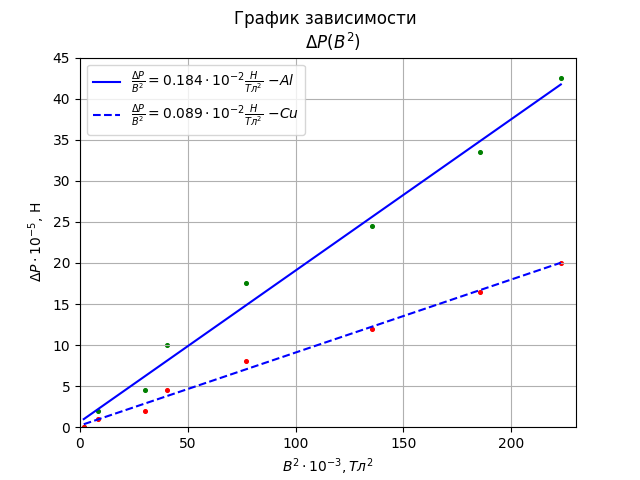
\includegraphics [scale=1]{3-4-1_second.png}}
		\caption{График зависимости $\Delta P (B^2)$}
	\end{figure}
	
	\newpage
	
	\textbf{Обсуждение результатов: }\\
	
	В данной работе мы определили значения магнитной восприимчивости $\chi$ двух образцов: диа- и парамагнетиков на примере медного и алюминиево стержней.
	Однако полученные значения $\chi$ больше табличных $\approx$ в 3 раза ($\chi_{Al} = 2,2 \cdot 10^{-5}$,   $\chi_{Cu} = -9,6 \cdot 10^{-6}$ - табличные данные)
	Наибольший вклад в погрешность $\chi$ внесла погрешность измерения магнитного потока $\Phi$, так как измерения проводились на стрелочном миливеберметре, а показания находились в первой половине шкалы из-за чего относительная погрешность измерений была высока.\\
	
	\textbf{Выводы: }\\
	
	В ходе работы мы смогли определить магнитную восприимчивость диа- и парамагнетиков методом Гюи, но полученные результаты отличаются от табличных. 

\end{document}